\documentclass[12pt]{article}

\usepackage[utf8]{inputenc}
\usepackage{listings}
\usepackage{graphicx}
\usepackage{float}
\usepackage{geometry}

\usepackage{parskip}
\setlength{\parskip}{1.0\baselineskip plus2pt minus2pt}

\addtolength{\topmargin}{-50pt}
\addtolength{\textheight}{130pt}
\addtolength{\textwidth}{95pt}
\addtolength{\oddsidemargin}{-45pt}

\title{Simulação e Computação Científica - Trabalho 1}
\author{David Gomes (2013136061), Nuno Gonçalves (2012139146), Marta Mercier (2013136742)}
\date{Março 2015}

\begin{document}
\maketitle

O primeiro trabalho de Simulação e Computação Científica consiste num ecossistema
descrito por uma grelha bidimensional, habitado por lobos e ovelhas.

Ao simularmos o ambiente, implementado em Java, detetamos que tanto os lobos como
as ovelhas morriam prematuramente (os lobos extinguiam-se depois de mais ou menos
700 iterações). Assim, encontramos valores mais apropriados para a simulação, de
forma a que haja sempre lobos e ovelhas durante as 5000 unidades de tempo.

Os valores que alteramos foram a probabilidade de reprodução das ovelhas, que aumentamos
de \texttt{0.04} para \texttt{0.10} e a energia ganha pelos lobos ao comer uma ovelha, que
diminuimos de \texttt{20} para \texttt{6}.

Apresentamos, de seguida, os diferentes gráficos do número de ovelhas de acordo com os valores do
enunciado e de acordo com os valores que alteramos.

\section{Valores do Enunciado}

\begin{figure}[H]
  \centering
  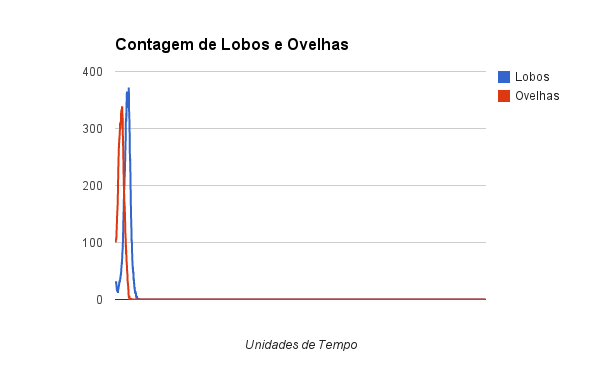
\includegraphics[width=0.75\textwidth]{ovelhaslobos1}
  \caption{Distribuição de Lobos e Ovelhas}
\end{figure}

A partir deste gráfico não é possível tirar grandes conclusões em relação
à evolução dos lobos e das ovelhas.

\begin{figure}[H]
  \centering
  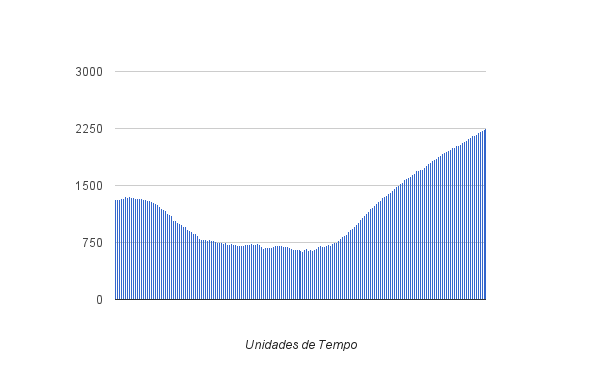
\includegraphics[width=0.75\textwidth]{vegetacao1}
  \caption{Evolução da Vegetação, em unidades}
\end{figure}

\section{Valores Alterados}

\begin{figure}[H]
  \centering
  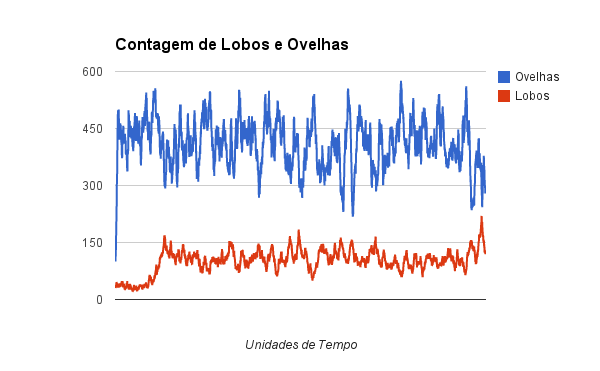
\includegraphics[width=0.75\textwidth]{ovelhaslobos2}
  \caption{Distribuição de Lobos e Ovelhas}
\end{figure}

Podemos notar, neste gráfico, o rápido crescimento do número de ovelhas nas primeiras iterações
da simulação devido ao aumento da probabilidade de reprodução destas.

\begin{figure}[H]
  \centering
  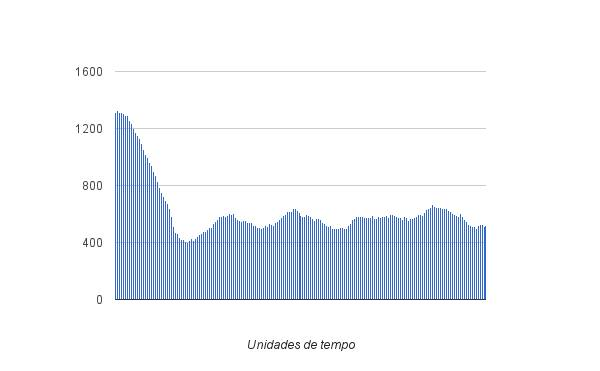
\includegraphics[width=0.75\textwidth]{vegetacao2}
  \caption{Evolução da Vegetação, em unidades}
\end{figure}

\section{Análise de Resultados e Conclusão}

Podemos concluir, comparando os gráficos da evolução da vegetação entre os dois
\textit{datasets}, que a vegetação é muito mais constante com os valores alterados.
Isto acontece porque a falta de ovelhas faz com que a vegetação cresça linearmente.


\end{document}
